%----------------------------------------------------------------------------------------
%	PACKAGES AND OTHER DOCUMENT CONFIGURATIONS
%----------------------------------------------------------------------------------------
\documentclass[11pt]{article}
\usepackage[english, french]{babel}
\usepackage[utf8]{inputenc}
\usepackage{graphicx}

% Used to format pars, specify the indent size and jump after par ending
\usepackage[skip=10pt plus1pt, indent=25pt]{parskip}

% Used to allow n-depth level for titles (pars become numbered). 
\usepackage{titlesec}
\setcounter{secnumdepth}{5}

% Hyphenation for languages with accented characters 
% is the main reason that requires T1 font encoding.
\usepackage[T1]{fontenc}

% Package used to create glossaries, acronym list...
\usepackage[acronym]{glossaries}

\makenoidxglossaries

\newacronym{esn}{ESN}{Entreprise de Services Numériques}
\newacronym{fyw}{FYW}{Find Your Way}
\newacronym{ea}{EA}{État de l'art}
\newacronym{jds}{JDS}{Journée des stagiaires}
\newacronym{rgbd}{RGB-D}{Red, Green, Blue and Depth}
\newacronym{imu}{IMU}{Inertial Measurement Unit}
\newacronym{slam}{SLAM}{Simultaneous Localization and Mapping}
\newacronym{cnn}{CNN}{Convolutional Neural Network}
\newacronym{vio}{VIO}{Visual-Inertial Odometry}
\newacronym{fast}{FAST}{Features from accelerated segment test}
\newacronym{orb}{ORB}{Oriented \acrshort{fast} and Rotated BRIEF}
\newacronym{cpu}{CPU}{Central Processing Unit}
\newacronym{gpu}{GPU}{Graphical Processing Unit}
\newacronym{tsdf}{TSDF}{Truncated Signed Distance Fields}
\newacronym{icp}{ICP}{Iterative Closest Point}
\newacronym{brief}{BRIEF}{Binary Robust Independent Elementary Features}
\newacronym{vm}{VM}{Virtual Machine}
\newacronym{wsl2}{WSL2}{Windows Subsystem for Linux 2}
\newacronym{poi}{POI}{Point of Interest}
\newacronym{poc}{POC}{Proof of Concept}
\newacronym{dbow2}{DBoW2}{Dynamic Bag of Words}
\newacronym{ros}{ROS}{Robot Operating System}
\newacronym{cv}{CV}{Computer Vision}
\newacronym{nlp}{NLP}{Natural Language Processing}

% Used to manage hyperlinks and make a clickable table of contents.
\usepackage{hyperref}
\hypersetup{
    colorlinks,
    citecolor=blue,
    filecolor=red,
    linkcolor=black,
    urlcolor=blue
}

% Used to create a bibliography using a .bib file.
\usepackage[
   backend=biber,
   style=numeric,
   sorting=nyt,
   url=true,
   doi=true,
   isbn=false,
]{biblatex}
\usepackage{csquotes}

\defbibenvironment{bibliography}
  {\begin{enumerate}}
  {\end{enumerate}}
  {\item}

\addbibresource{PFE.bib}

% Defines graphics path.
\graphicspath{ {./images/} }

% Defines a new command for the horizontal lines, change thickness here.
\newcommand{\HRule}{\rule{\linewidth}{0.5mm}} 

\begin{document}

  \begin{titlepage}   
    % Center everything on the page.
    \center 

    %----------------------------------------------------------------------------------------
    %	LOGO SECTION
    %----------------------------------------------------------------------------------------

    \begin{figure}[!tbp]
      \centering
      \begin{minipage}[t]{0.4\textwidth}
        
\includegraphics[width=\textwidth]{Logo_ESIEA.jpg}    
      \end{minipage}
      % \hfill is used to evenly distribute the logos
      \hfill 
      \begin{minipage}[t]{0.4\textwidth}
        
\includegraphics[width=\textwidth]{Logo_Aubay.jpg}    
      \end{minipage}
    \end{figure}

    %----------------------------------------------------------------------------------------
    %	TITLE SECTION
    %----------------------------------------------------------------------------------------

    % Black horizontal line.
    \HRule \\[0.4cm]
  
    { \huge \bfseries Mission de fin d’études}\\ 
    % Space below "Mission de fin d'étude.
    \vspace{5ex}
    { \huge \bfseries Find Your Way}
    
    \HRule \\[0.8cm]
    \textsc{\LARGE Aubay}\\[1.5cm]
    
    %----------------------------------------------------------------------------------------
    %	AUTHOR SECTION
    %----------------------------------------------------------------------------------------

    \begin{minipage}{0.4\textwidth}
      \begin{flushleft} \large
        \emph{Maître de stage:} \\
        Nathan  \textsc{CANTAT} 
      \end{flushleft}
    \end{minipage}
    ~
    \begin{minipage}{0.4\textwidth}
      \begin{flushright} \large
        \emph{Jury de stage:} \\
        Arnaud  \textsc{BANNIER} 
      \end{flushright}
    \end{minipage}\\[2cm]
    
    \begin{minipage}{0.4\textwidth}    
      \emph{Auteur:}\\
      \bfseries \Large Nicolas \textsc{Cisternas}      
    \end{minipage}\\[2cm]

    %----------------------------------------------------------------------------------------
    %	DATE SECTION
    %----------------------------------------------------------------------------------------

    \large 28 février - 31 août 2022

  \end{titlepage}

  % Used to write the abstract in french.
  \selectlanguage{french} 
  \begin{abstract}
    % TODO: Abstract à terminer.

    Le projet Find Your Way a pour but de guider des personnes malvoyantes en milieu intérieur. Ce document relate le travail éffectué autour
    de cette thématique dans le cadre de mon stage de fin d'études, en se focalisant sur la partie localisation et guidage de l'utilisateur.
    Un état de l'art concernant le sujet de la localisation et de la cartographie locale en temps réel est présenté. Ensuite une preuve de
    concept se basant sur une méthode en sources libres, contenant les améliorations que mon groupe et moi avons pu ajouter est expliquée 
    dans ce document. Enfin ce document explique le déroulement de la phase projet au sein de la cellule Innov' de l'entreprise Aubay
    pour démontrer le résultat d'une collaboration entre 11 stagiaires. Le lecteur pourra y trouver des informations concernant ORB-SLAM3,
    FAST, les points d'intérets, la création d'un protocole de communication, le développement de l'interface graphique et les problèmes 
    que l'on peut rencontrer sur ce genre de projet multidisciplinaire.

  \end{abstract}
  \pagebreak

  % Used to write the abstract in english.
  \selectlanguage{english} 
  \begin{abstract}
  % TODO: Abstract en anglais à écrire.
    Abstract in English
  \end{abstract}
  \pagebreak

  \selectlanguage{french} 
  \setcounter{tocdepth}{3}
  \tableofcontents

  \pagebreak

  \section{Remerciements}    
    Je remercie Éric REMILLERET et Nathan CANTAT, mes maîtres de stage, 
    ainsi que Wael NASR, pour m'avoir donné l'opportunité de rejoindre 
    Aubay Innov', qui s'est avérée être une expérience intéressante 
    et instructive, ainsi que pour l'aide à la relecture de ce rapport.    
    
    Je remercie Anne-France GALLAND, qui a largement contribué à la phase de suivi et d'organisation du projet, par ses interventions 
    lors des réunions hebdomadaires et pour le temps qu'elle a pris pour la relecture de ce rapport.    
    
    Je remercie Jean-Philipe CUNNIET, mon tuteur de stage ainsi qu'Arnaud BANNIER, le jury de cette mission de fin d'études, 
    pour le temps qu'ils ont passé à relire et évaluer ce rapport de stage ainsi que la soutenance de stage.    

    Je tiens à remercier toute l'équipe avec laquelle j'ai 
    travaillé durant mon stage:    
    Nicolas GUILLERMAIN et Mathieu MONNERET avec qui j'ai travaillé lors 
    de la phase d'état de l'art et de preuve de concept.
    Mélissa WANG et Jeoffrey MENUDIER avec qui j'ai principalement 
    travaillé lors de la phase projet. 
    Jean-Baptiste CHANIER, Victor CHAVEROT, Jean-Noël CLINK,
    Ophélie PHONCHAREUN, Miora RASOLOFONERA et Rémi VIDAL avec qui j'ai échangé tout au 
    long du stage concernant leurs parties du projet.       
    
    Je tiens également à remercier la direction générale d'Aubay pour leur accueil et leur écoute ainsi qu'Ophélie CHEVALIER, campus manager, 
    pour tous les événements qu'elle a pu organiser et qui ont permis d'établir un climat chaleureux entre les différents groupes.
        
    Enfin, je remercie les autres étudiants d’Aubay Innov' avec lesquels j'ai eu l'occasion d'échanger aussi bien humainement que techniquement.

  \pagebreak

  \section{Introduction et contexte}    
  
    Mon stage s'est déroulé dans une entreprise appelée Aubay, pour une durée de 6 mois (du 28 février 2022 au 31 août 2022). 
    En détail, Aubay est une entreprise de services numériques (\acrshort{esn}) qui a été fondée par Christian Aubert en 1998 et 
    dont le siège social est situé au 13 rue Louis Pasteur à Boulogne-Billancourt. L'entreprise est spécialisée dans les domaines 
    liés à la finance, à l'assurance et à la banque et est également impliquée dans divers marchés, tels que les télécoms, 
    les services, les réseaux, l'énergie et les transports. Aubay accompagne la transformation et la modernisation des systèmes 
    d’information de ses clients. Ils opèrent sur des marchés à forte valeur ajoutée, en France comme en Europe. C'est un acteur 
    référent de la transformation digitale. Son secteur d'activité est centré autour du conseil sur tout type de projet technologique.  
    C'est une ESN cotée en Bourse (SBF 250) et 46\% du capital est détenu par les managers. Les chiffres clés concernant Aubay 
    sont présentés dans la Figure \ref{fig:PA1} ci-après. En 2022, l'entreprise emploie 7306 travailleurs, dont 2728 en France. 
    Selon son site internet, Aubay est implantée dans 7 pays européens, et a réalisée un chiffre d'affaires de 470,6 M€ en 2021. 
    D'ailleurs, ces dernières années, l'entreprise a connu une forte croissance de 10,4\% en 2021, qui coïncide avec une augmentation 
    constante des effectifs de l'entreprise, passant de 4600 employés en 2015 à plus de 7000 aujourd'hui.
  
    \begin{figure}[hbt]  
      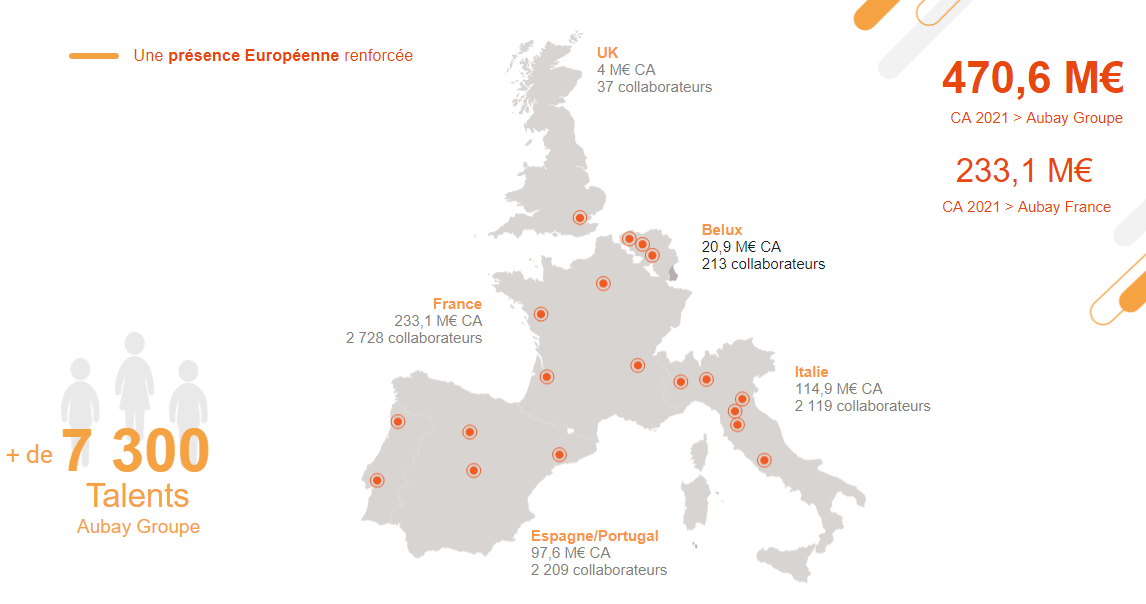
\includegraphics[width=\textwidth]{PresentationAubay1.png}    
      \caption{Chiffres clés pour Aubay en 2021.}
      \label{fig:PA1}
    \end{figure}    
    
    J'ai eu le privilège d'effectuer mon stage au sein de l'unité "Aubay Innov'" qui est la division d’Aubay France dédiée 
    à la recherche et à l'innovation. Ses membres sont impliqués dans différents projets, chacun lié à la data science, l'analyse 
    de données ou tout autre domaine liés aux nouvelles technologies numériques. L'objectif de l'unité est d'acquérir 
    les connaissances et le savoir-faire pour construire des solutions durables et innovantes adaptées aux besoins futurs des clients. 
    Les projets dirigés dans la cellule innovation d'Aubay ne sont donc soumis à aucun client pendant leur réalisation, 
    ce qui laisse l'opportunité aux stagiaires d'expérimenter autant qu'ils le souhaitent durant leur stage.
    Chaque année, cette unité donne la chance à des dizaines de stagiaires d'améliorer ou de perfectionner leurs connaissances
    relatives à la science des données en leur laissant l'opportunité de découvrir et d'expérimenter les technologies les plus 
    innovantes disponibles dans les domaines de la recherche. Par ailleurs, l'unité "Aubay Innov'" est largement considérée comme 
    une source de recrutement pour l'entreprise, qui a souhaité cette année engager environ 800 nouveaux collaborateurs en France. 
    
    C'est dans ce cadre que ma mission de fin d'études a débuté. Le projet "Find Your Way" (\acrshort{fyw}), qui représente l'expérience que je 
    vais détailler dans ce document, a été lancé en février 2022 et a pour objectif de créer une application embarquée sur des lunettes, 
    basée sur des algorithmes capables de reconnaître les éléments de l'environnement immédiat d'un utilisateur malvoyant pour le guider 
    vers des lieux ou l'avertir d'obstacles présents sur son chemin tels que des chaises ou une personne par exemple. Un objectif majeur 
    de ce projet est également de localiser l'utilisateur dans son environnement afin de lui permettre de retrouver son chemin jusqu'à
    un endroit précédemment enregistré et de le guider avec des indications de direction et d'orientation dans ses déplacements en intérieur
    en temps réel, le tout répondant à un système de commandes vocales.  
    
    Les systèmes d'aide automatisés au déplacement de personnes malvoyantes existent déjà sur le marché et nécessitent de fournir une 
    carte du bâtiment avec les lieux importants préalablement renseignés afin de rendre le guidage possible. Ce projet vise à s'affranchir 
    de cette contrainte afin de permettre une plus grande polyvalence pour ce genre d'outil.
    Le projet a été séparé en plusieurs parties délimitées par des dates clés qui sont présentées dans la Figure \ref{fig:Planning} 
    avec les livrables associés à chaque fin de phase.
    La prise en main du projet a démarée début février, s'en est suivi la partie concernant les états de l'art (\acrshort{ea} sur la Figure \ref{fig:Planning}) 
    qui devait être réalisée entre mi-février et mi-mars en parallèle du Design Thinking qui nous a permis de cadrer et définir le projet par 
    rapport aux besoins de l'application et les tâches à accomplir. La phase de preuve de concept qui a suivi a duré jusqu'à mi-mai. 
    Une fois ces étapes réalisées nous avons pu passer à la phase projet afin de réunir toutes les preuves de concept et concevoir l'application 
    de démonstration nécessaire à la journée des stagiaires (\acrshort{jds}) du 7 juillet, moment phare pour le pôle innovation de chez Aubay où tous 
    les stagiaires présentent leurs projets lors d'une démonstration auprès des directeurs généraux et directeurs commerciaux de l'entreprise.

    \begin{figure}[hbt]  
      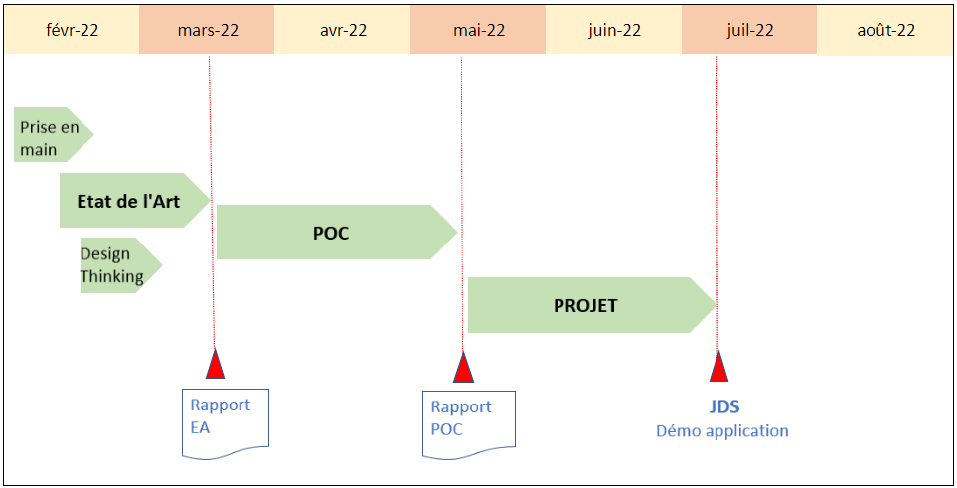
\includegraphics[width=\textwidth]{Planning.png}    
      \caption{Planning prévisionnel du projet \acrshort{fyw}.}
      \label{fig:Planning}
    \end{figure}  
    
    J'ai réalisé ce projet dans une équipe de 11 stagiaires, tous en stage de fin d'études. Étant donné les multiples parties concernant le projet, 
    à savoir la détection d'objets, la localisation de l'utilisateur et la gestion des interactions vocales, nous avons dû nous séparer en 3 
    groupes afin de réaliser les états de l'art et les preuves de concept. J'ai personnellement travaillé sur la partie s'intéressant à la 
    localisation et le guidage de l'utilisateur dans son environnement. 
    \pagebreak
  
  \section{État de l'art}  

    \subsection{Recherches bibliographiques}
      Dans cette section je présente les recherches bibliographiques que j'ai pu effectuer avec mon groupe lors de la phase d'état de l'art.
      Cet état de l'art concerne la partie de localisation et de guidage de l'utilisateur. Nous avons retenu 8 publications, nous les avons 
      confrontées et comparées afin de n'en sélectionner qu'une sur laquelle nous allions nous concentrer lors de la phase de preuve de 
      concept. Je présente ici 4 des publications les plus pertinentes sur le sujet.
      
        \subsubsection{Wearable Travel Aid for Environment Perception and Navigation of Visually Impaired People}
          L'appareil consiste en une caméra grand public rouge, vert, bleu avec de la profondeur (\acrshort{rgbd} pour red, green, blue, depth)
          et une unité de mesure inertielle (\acrshort{imu} pour Inertial Measurement Unit), c'est un capteur qui consiste généralement en des gyroscopes 
          pour mesurer des vitesses angulaires et des accéléromètres pour mesurer la force \cite{baiWearableTravelAid2019}. Ces appareils sont montés sur une paire de lunettes
          et reliés à un téléphone. L'appareil proposé dans cette solution se sert de la continuité de la hauteur du sol entre les images 
          adjacentes poursegmenter le sol avec précision et rapidité pour ensuite chercher la direction du mouvement en fonction du sol.
          Un réseau de neurones à convolution (\acrshort{cnn} pour Convolutional Neural Network) léger est utilisé pour la reconnaissance d'objets 
          (PeelNet avec l'ensemble de données "MS COCO" contenant des images de dimensions 640 x 640). Son schéma de fonctionnement est présenté 
          dans la figure \ref{fig:ReconnaissanceP1}. Il permet de récupérer des informations concernant les endroits aux alentours et l'orientation 
          des objets environnants. Le schéma de fonctionnement du système est présenté dans la Figure \ref{fig:PipelineP1}.

          \begin{figure}[hbt]  
            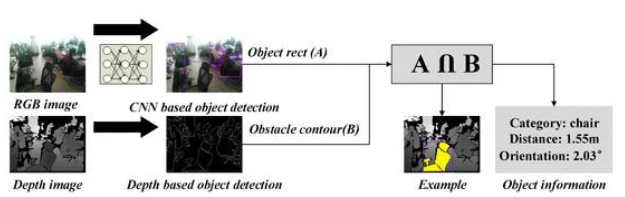
\includegraphics[width=\textwidth]{RecognitionP1.png}    
            \caption{Schéma présentant le fonctionnement du système de reconnaissance d'objets.}
            \label{fig:ReconnaissanceP1}
          \end{figure} 

          \begin{figure}[hbt]  
            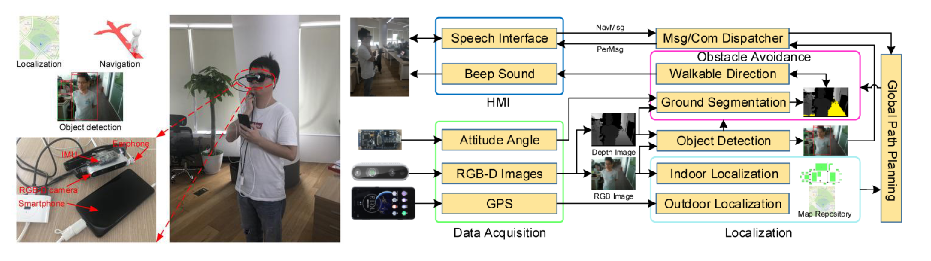
\includegraphics[width=\textwidth]{PipelineP1.png}    
            \caption{Schéma de fonctionnement du système proposé.}
            \label{fig:PipelineP1}
          \end{figure} 

          Le système de navigation contient un module de localisation intérieur qui va nous intéresser: un algorithme V\acrshort{slam} (Visual Simultaneous 
          Localization and Mapping) est utilisé. \acrshort{slam} est un problème de computer vision visant à traquer les mouvements d'un module en se basant
          sur ce qu'il voit. Il faut traiter les objets dynamiques qui entrent et sortent du champ de vision pour ne pas les prendre en computer
          dans l'estimation de la position du module. L'estimation se fait en trouvant des points clés sur les images successives.  Visual \acrshort{slam}
          se sert des informations récuperées pour trianguler la position 3D du module. 
    
        \pagebreak

        \subsubsection{CDSFusion: Dense Semantic SLAM for Indoor Environment Using CPU Computing}
          La solution CDSFusion \cite{wangCDSFusionDenseSemantic2022} se sert d'images RGB comme l'article précédent ainsi qu'un capteur \acrshort{imu} comme paramètres d'entrée et est composée de 
          3 modules imagés dans la Figure \ref{fig:PipelineP2}:

          \paragraph{Le module VIO}
            Le module d'odométrie visuelle-innertielle (\acrshort{vio} pour Visual-Inertial Odometry) se sert des entrées pour estimer avec précision la position 
            afin de proposer une trajectoire. Ce module \acrshort{vio} est basé sur VINS-Mono. VINS-Mono est un framework \acrshort{slam} en temps réel pour les 
            systèmes visuo-inertiels monoculaires. Il utilise une méthode de fenêtre glissante basée sur des optimisations pour fournir une odométrie 
            visuelle-inertielle de haute précision.
            Les features \acrshort{fast} (Features from accelerated segment test) ont été adaptées pour accélérer le \acrshort{vio} à 
            la place des feature Shi-Thomas (une manière de détecter les coins sur une image) et la profondeur a été introduite afin d'obtenir une échelle 
            plus précise. Les résultats expérimentaux montrent que les features \acrshort{fast} augmentent la rapidité du système d'une manière plus conséquente 
            que les features Shi-Tomas et \acrshort{orb} avec la même précision et robustesse. Ce module est composé de 3 parties:

          \underline{Visual-Inertial Frontend: }
            prend en charge le traitement des données issues des capteurs. Les mesures effectuées par le capteur \acrshort{imu}
            sont préintégrées entre deux images consécutives, le frontend de vision détecte les \acrshort{fast}
            et les traque entre les images consécutives en utilisant l'algorithme KLT optical flow.

          \underline{Back-End:} est utilisé pour fusionner les mesures traitées afin d'obtenir l'estimation de la position. Une optimisation non linéaire
            est utilisée pour relocaliser et optimiser le calcul de la position en fonction de la boucle détectée, en utilisant le solveur Ceres. 

          \underline{Le module de détection de boucle: } permet de relocaliser et optimiser le calcul de la position en fonction de
            la boucle détectée. En effet, une boucle est détectée lorsque l'on a réalisé une boucle dans le parcours d'un chemin, il devient alors inutile
            de recalculer la position tant que l'utilisateur se situe dans cette boucle, on peut alors facilement optimiser le calcul de la position en se 
            basant sur des calculs précédemment effectués. Cela se base sur la bibliothèque Dynamic Bag of Words (\acrshort{dbow2}) qui est à l'état de l'art de la reconnaissance d'endroits 
            par sac de mots (bag of words approach). De même, lorsqu'une boucle est détectée, une optimisation est possible pour le calcul de la position 
            globale. Cette optimisation est similaire à la méthode VINS-Mono.

          \paragraph{Le module de segmentation sémantique}
            La segmentation sémantique résulte d'images RGB en entrée qui sont acquises en temps réel en utilisant le module de segmentation PSPNet. 
            Le module de segmentation sémantique traite chaque image RGB et retourne des vecteurs indiquant la probabilité d'appartenance à une classe
            pour chaque pixel. Ils classifient et colorent chaque pixel en fonction de la plus haute probabilité d'appartenance à une classe. 
            L'image segmentée finale est composée des pixels colorés et est transmise au module de reconstruction 3D.

          \paragraph{Le module de reconstruction 3D}
            Le nuage sémantique local est généré en utilisant une image sémantique (générée par le module précédent) et une carte de profondeur. 
            Ce nuage local servira à produire un nuage global une fois qu'il sera combiné avec les estimations de position de la caméra depuis le module \acrshort{vio}.
            Pour construire une carte 3D globale qui soit précise, un modèle basé sur des voxels est utilisé pour filtrer le bruit et extraire un mesh global.
            À chaque image importante (Keyframe), la carte de profondeur courante est transformée en nuage de points 3D, ensuite les options Voxblox et \acrshort{fast}
            sont adaptées, le nuage local de points 3D est transformé en mesh local et ensuite ce mesh local est intégré dans le mesh global. L'ensemble de 
            cette procédure est réalisée en temps réel sur \acrshort{cpu}. Voxblox est une bibliothèque de cartographie volumétrique basée principalement 
            sur les \acrshort{tsdf} (Truncated Signed Distance Fields).

            \begin{figure}[hbt]  
              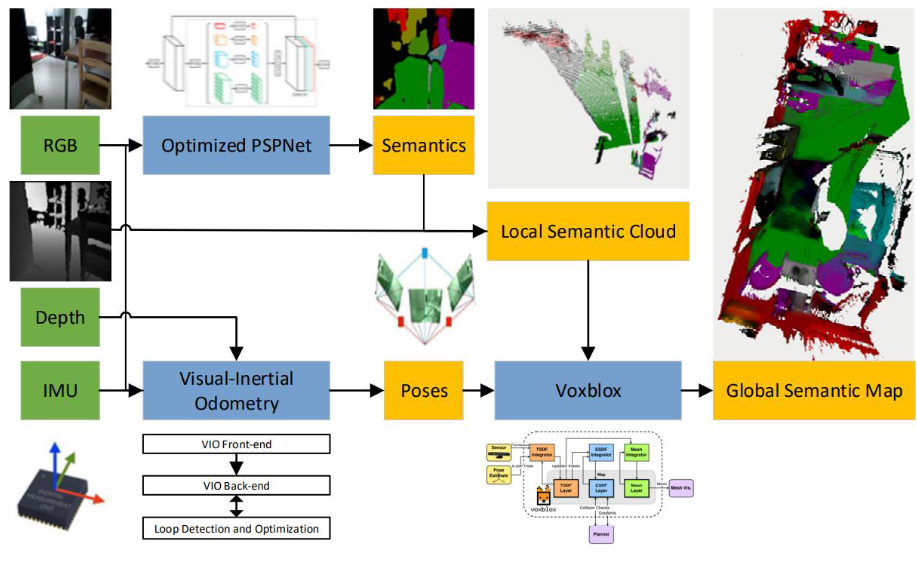
\includegraphics[width=\textwidth]{PipelineP2.png}    
              \caption{Schéma présentant le fonctionnement du système proposé.}
              \label{fig:PipelineP2}
            \end{figure} 
          
        \pagebreak  

        \subsubsection{Towards Real-time Semantic RGB-D SLAM in Dynamic Environments} 
          Cet article \cite{jiRealtimeSemanticRGBD2021} présente une méthode de \acrshort{slam} s'inspirant des features \acrshort{orb} (Oriented \acrshort{fast} and Rotated \acrshort{brief}).
          Le module de segmentation sémantique est une adaptation de SegNet, un réseau de neurones léger qui permet un traitement en temps réel.
          La segmentation se concentre sur des objets dynamiques dont les caractéristiques ne seront pas utilisées dans la création de 
          la carte locale. La segmentation est faite uniquement sur les images clés les plus récentes, accélérant grandement le processus.
          La segmentation peut être très rapide, mais reconnaît principalement les objets qu'elle connaît déjà et est moins efficace dans des 
          milieux inconnus avec des objets dynamiques nouveaux. Ce module essaye de résoudre ce problème.
          Pour chaque nouvelle image l'idée est d'utiliser l'algorithme du K-means pour segmenter l'image de profondeur en N clusters.
          Chaque cluster est considéré comme faisant partie du même objet. Pour chaque cluster, une erreur de reprojection est calculée. Si une 
          des erreurs moyennes est relativement supérieure aux autres, le cluster est considéré comme un objet dynamique et les points caractéristiques
          de l'objet seront supprimés du traitement. Cette manière de traiter les images permet de réduire le taux de faux positifs. 
          Les comparaisons sont effectuées d'une image clé à une autre puisqu'elles se ressemblent beaucoup, mais aussi entre la première estimation
          et les cartes locales obtenues.

        \pagebreak

        \subsubsection{ORB-SLAM3: An Accurate Open-Source Library for Visual, Visual-Inertial and Multi-Map SLAM}
          \acrshort{orb}-SLAM3 \cite{camposORBSLAM3AccurateOpenSource2021} est une amélioration d'\acrshort{orb}-\acrshort{slam}2, présenté 
          en Figure \ref{fig:ORBSLAM2}, qui consistait à travailler sur trois tâches simultanément : 
          le suivi, la cartographie locale et la fermeture de boucle. Dans sa partie de suivi, \acrshort{orb}-\acrshort{slam}2 fait correspondre les caractéristiques image 
          par image et les compare avec une carte locale pour trouver l'emplacement exact de la caméra en temps réel. Il procède à un ajustement 
          en fonction du mouvement afin de minimiser l'erreur de reprojection. Vient ensuite la partie cartographie locale 
          dans laquelle \acrshort{orb}-\acrshort{slam}2 
          créer des cartes locales et les optimise en utilisant des algorithmes tels que Iterative Closest Point (\acrshort{icp}) et effectue un ajustement 
          local afin de calculer la position la plus probable de la caméra. Enfin, il utilise l'optimisation du graphe des positions 
          pour corriger la dérive accumulée et effectuer une fermeture de boucle. Il est nécessaire d'effectuer un ajustement groupé
          après la fermeture de la boucle, afin que l'utilisateur se trouve à l'emplacement le plus probable dans la carte corrigée. 
          Après l'ajout d'une image clé à la carte ou l'exécution d'une fermeture de boucle, 
          \acrshort{orb}-\acrshort{slam}2 peut démarrer un nouveau fil d'exécution qui effectue un ajustement de l'ensemble de la carte afin que 
          l'emplacement de chaque image clé et des points dans celle-ci obtienne une valeur d'emplacement ajustée.

          Pour traiter une image \acrshort{rgbd}, on calcule d'abord les caractéristiques \acrshort{orb} sur l'image RGB, ensuite on estime les coordonnées de l'image de 
          gauche depuis une paire d'images. Un point est associé à "proche" ou "éloigné" en fonction de sa profondeur. Chaque dénomination a des
          caractéristiques utiles, un point proche sera représentatif pour le changement d'échelle, la translation, la rotation alors qu'un point éloigné
          sera surtout utile pour la rotation et devra être supporté par un plus grand nombre d'images.
          À l'initialisation, le système nécessite seulement les premières images clés pour estimer la première carte locale en utilisant les informations
          de profondeur. 
          L'insertion d'une nouvelle image clé est importante, car elle définit le nouvel environnement sur lequel se base l'estimation du mouvement 
          de la caméra. Elle suit l'idée établie par la première version d'\acrshort{orb}-\acrshort{slam}, d'insérer régulièrement de nouvelles images clés, 
          même si cela implique de devoir les retirer si elles sont redondantes. L'ajout de points clés proches et éloignés permet un nouveau seuil 
          d'apparaître pour déterminer si une nouvelle image clé est nécessaire. 
          Si le nombre de points proches devient inférieur à un seuil, il sera nécessaire d'insérer une nouvelle image clé comportant au moins un certain
          nombre de points proches supérieur à un autre seuil.

          \begin{figure}[hbt]  
            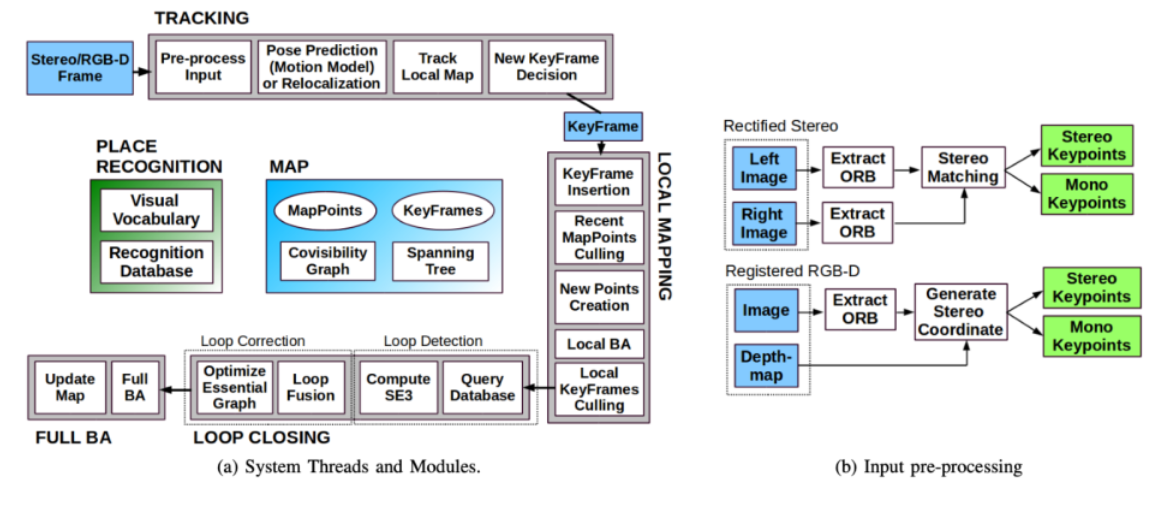
\includegraphics[width=\textwidth]{ORB_SLAM2.png}    
            \caption{Schéma présentant le fonctionnement d'\acrshort{orb}-SLAM2.}
            \label{fig:ORBSLAM2}
          \end{figure} 

          \acrshort{orb}-SLAM3 introduit l'utilisation de mémoire à court, moyen et long terme regroupées dans un Atlas.
          En se servant des données que l'on a déjà vues, on peut retrouver
          facilement les boucles et ainsi réduire les erreurs de dérive. Une représentation en sac de mot dynamique (DBoW2) est utilisée.
          Ce système est présenté en Figure \ref{fig:ORBSLAM3}

          \begin{figure}[hbt]  
            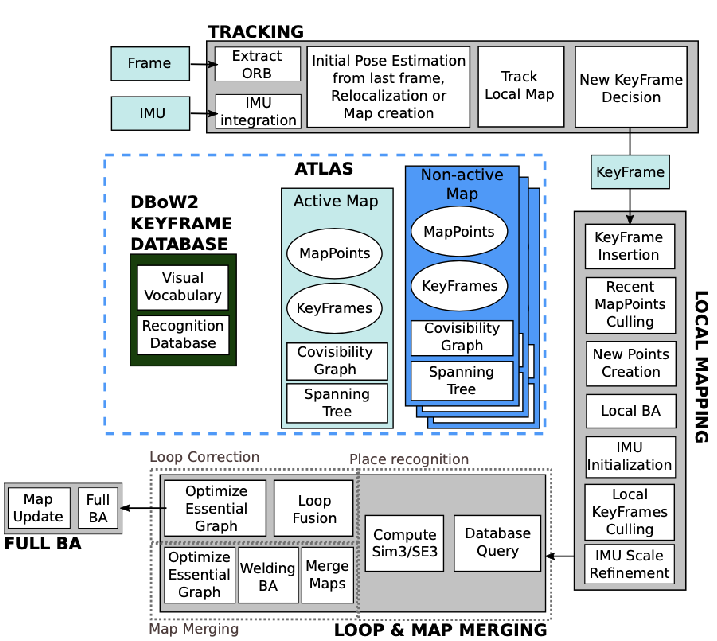
\includegraphics[width=\textwidth]{ORB_SLAM3.png}    
            \caption{Schéma présentant le fonctionnement d'\acrshort{orb}-SLAM3.}
            \label{fig:ORBSLAM3}
          \end{figure} 

          Le thread de tracking traite chaque nouvelle image afin de vérifier si elle représente une nouvelle image clé afin de la localiser
          dans la carte active de l'atlas. Si le tracking est perdu, le système essaye de se relocaliser en cherchant des repères visuels 
          qu'il a déjà rencontrés par le passé. Si cela ne fonctionne pas, il créera une nouvelle carte qui sera la nouvelle carte active dans l'atlas.
          On dispose donc d'un atlas de cartes locales, un ensemble de cartes déconnectées qui seront peut-être combinées avec le temps grâce au 
          système de fermeture de boucles.

        \pagebreak

    \subsection{Synthèse}
      L'article "Wearable Travel Aid for Environment Perception and Navigation of Visually Impaired People" est très détaillé et demande beaucoup 
      de temps pour saisir chaque subtilité.
      Au début de l'article, les auteurs listent les solutions qui existent déjà et expliquent leurs limitations respectives. 
      Chaque partie de la solution est expliquée et peut être trouvé dans leur travaux précédents. Cette solution prendrait beaucoup de temps
      à implémenter puisque les auteurs font surtout une description de leur travail sans mettre à disposition de code source. 
      Il faudrait parcourir tous leurs travaux précédents pour comprendre l'intégralité de leur solution. De plus il faudrait adapter les travaux
      proposés afin de créer la carte locale en temps-réel plutôt qu'avant, puisque c'est une des contraintes imposées par nos superviseurs. 

      L'article "CDSFusion : Dense Semantic \acrshort{slam} for Indoor Environment Using \acrshort{cpu} Computing" est très prometeur mais n'est pas assez détaillé 
      pour nous permettre de reproduire leur solution à partir de rien. De plus ils utilisent des capteurs \acrshort{imu}, que nous avons convenu de ne pas 
      utiliser dans le cadre de ce projet.

      L'article "Towards Real-time Semantic \acrshort{rgbd} \acrshort{slam} in Dynamic Environments" apporte une solution de tracking de la localisation 
      d'un module en temps réel, ce qui correspond à ce que l'on recherche dans le cadre de ce projet. Cette solution aide à garder en 
      mémoire les directions prises jusqu'à arriver à un point donné. Cependant les auteurs ne parlent que peu d'\acrshort{orb}-\acrshort{slam} et se focalisent 
      surtout sur leur valeur ajouté permettant d'améliorer les résultats de ce dernier.

      Enfin, l'article "\acrshort{orb}-\acrshort{slam}3 : An Accurate Open-Source Library for Visual, Visual-Inertial and Multi-Map \acrshort{slam}" semble être le plus abouti
      que nous aillons pu lire, il est à l'état de l'art et obtient de meilleurs performances que ses concurants. L'article est assez bien expliqué
      et fourni un code source disponible sur Github. Leur solution semble réutilisable pour notre problème, cela apporterait un bon moyen
      de traquer une personne malvoyante dans une pièce. Certains aspects de la publication semblent compliqués à comprendre mais la méthode en 
      elle même nous semble accessible. Il faudrait passer du temps sur leur code source afin de l'appréhender et se rendre compte de la faisabilité
      de sa mise en place.

    \pagebreak

    \subsection{Conclusion}
      Pour conclure sur cet état de l'art, nous avons découvert plusieurs méthodes permettant de traquer le mouvement d'une caméra dans un
      milieu intérieur, chacune avec son niveau de complexité et de faisabilité par rapport à nos contraintes qui étaient de n'utiliser aucun
      autre capteur qu'une camera. Notre but final était de fournir un module permettant de guider une personne d'un point A à un point B avec 
      l'aide de notre module créant une carte locale de l'environnement en se basant sur des points et des lieux d'intérêt, 
      s'emboîtant avec les modules de traîtement du langage naturel, et le module de détection d'objets. 
      L'article "\acrshort{orb}-\acrshort{slam}3 : An Accurate Open-Source Library for Visual, Visual-Inertial and Multi-Map \acrshort{slam}" 
      nous a semblé être le plus pertinent pour arriver à notre but. En effet nous pourrions nous baser sur leur solution de tracking et construire 
      par dessus pour répondre au besoin fonctionnel de ce projet.
      De plus le fait que les auteurs mettent à disposition leur code source donne une première vision de ce qui pourrait être réalisé en terme de 
      performances avec notre propre environnement.

    \pagebreak
  
  \section{Les dimensions techniques du projet (8 à 12 p)}
    Description des objectifs/tâches qui vous ont été confiés, vous exposerez les difficultés rencontrées et la manière dont vous
    les avez abordées.  Vous mettrez également en valeur l’originalité éventuelle de votre approche, les
    choix et décisions que vous aurez prises. Vous mettrez vos travaux et réalisations en perspective par
    rapport à l’ensemble du projet et son historique.

    \subsection{Phase de preuve de concept}
      Le projet \acrshort{fyw} vise à aider les personnes malvoyantes à se repérer en milieu intérieur. 
      La preuve de concept (\acrshort{poc}) sur laquelle j'ai travaillée avec mon équipe se concentrait sur la création d'une carte locale
      de l'environnement en nous basant sur des points d'intérêts (\acrshort{poi}) entre les images vues successivement, c'est la méthode
      \acrshort{slam}.
      \subsubsection{Installation}
        Il a d'abord fallu se pencher sur l'installation de la solution que nous avions retenue, afin de construire notre module par dessus.
        Nous avons été capable de produire une documentation d'installation de ORB-SLAM3 sur le Windows sub-system for Linux (\acrshort{wsl2})
        et sur une machine virtuelle (\acrshort{vm}). Ces documentations d'installation appartiennent à Aubay et ne peuvent être divulguées dans
        ce document.
        Ensuite il a fallu calibrer la caméra que nous utilisions pour fonctionner avec \acrshort{orb}-\acrshort{slam}3. 
        La calibration de la caméra assure que l'estimation de la position de la caméra est la plus proche de la position réelle de la caméra.
        Enfin, l'idée était de développer un algorithme de recherche du plus court chemin entre deux points donnés, par exemple entre la position
        de l'utilisateur et une destination précédemment sauvegardée.      
            
        \paragraph{General}
          Notre méthode se base sur ORB-SLAM3, une solution open-source crée dans une université en Espagne. L'idée était simple, nous voulions
          l'installer et la faire fonctionner puis ajouter les fonctionnalitées nécéssaires à notre \acrshort{poc}. Ce projet open-source a été
          développé en C++ et se base sur de nombreuses bibliothèques de code telles que Eigen, Pangolin, Sophus, DBoW2, g2o, Kalibr et ROS.
          Avant d'installer ORB-SLAM3 nous avons dû installer Eigen et Pangolin. Sophus, DBoW2 et g2o étant déjà inclus dans leur dépôt Github.

          Nous avons essayé d'installer \acrshort{orb}-\acrshort{slam}3 sur Windows 10, Mac OSX, Ubuntu 20.04 sur VirtualBox et enfin 
          \acrshort{wsl2}. L'installation sous Windows 10 a rapidement été déclarée impossible puisqu'\acrshort{orb}-\acrshort{slam}3
          a été développé pour un système Linux en grande majorité. L'installation sur Mac OSX n'a été que temporaire, le temps que l'on 
          obtienne l'autorisation de travailler avec \acrshort{wsl2}.
          Nous avons donc réalisé l'installation d'\acrshort{orb}-\acrshort{slam}3 sur \acrshort{wsl2} et réussi à lancer le \acrshort{slam}
          sur la vidéo d'exemple fournie. Cependant notre \acrshort{poc} devait fonctionner avec un flux vidéo en temps réel provenant
          d'une caméra, et non une vidéo préenregistrée. Le problème était que bien que wsl2 ai accès aux appareils USB (en prenant en compte 
          que pour cela il était nécéssaire de créer un noveau noyau Linux contenant les bons pilotes) et que la caméra soit visible dans les
          pilotes USB, le sous-système n'était pas capable de créer la vidéo dans /dev/video, rendant le flux vidéo innaccessible à notre
          application. Nous avons choisi de basculer sur un sysème Ubuntu 20.04 sur VM afin de disposer des fonctionnalités de base
          nécéssaires à notre avancée.     

        \paragraph{Eigen}
          Eigen est une bibliothèque d'algèbre linéaire, elle traîte les vecteurs, matrices, solveurs numériques et les algorithmes
          associés. Cette bibliothèque est nécéssaire au bon fonctionnement d'ORB-SLAM3. Pour l'installer, nous avons dû chercher la version 
          adaptée puisque la bibliothèque a évolué depuis la publication du dépot Github d'ORB-SLAM3, rendant les versions les plus récentes
          de Eigen incompatibles avec le projet. Nous avons essayé plusieurs versions qui n'ont pas fonctionnées jusqu'à déterminer que la version 
          3.3.1 était la version utilisée au moment du développement d'ORB-SLAM3.

        \paragraph{Pangolin}
          Pangolin est un ensemble de bibliothèques utilitaires légères traîtant de prototypage 3D et d'algorithmes numériques 
          ou basés sur de la vidéo. Elles sont utilisées pour s'affranchir des contraintes d'environnement et rendre facile la visualisation des 
          données. Pour l'installation, de même que pour Eigen, la version la plus récente ne correspondait pas alors il a fallu chercher dans 
          l'historique des versions et tester jusqu'à trouver la version 0.6 sur leur Github qui nous a permis de lancer le projet.

        \paragraph{ORB-SLAM3}
          Pour installer ORB-SLAM3, il a d'abord fallu cloner le dépôt Github de la version 1.0. 
          Il y avait des prérequis qui ne correspondaient pas à notre environnement tels que la version d'OpenCV qu'il a fallu adapter,
          nous avons déterminé que la version 4.2 était la bonne. Pour chaque bibliothèque nécéssaire nous avons du trouver la version
          adaptée à notre projet. Ensuite nous avons pu installer les bibliothèques tierces déjà contenue dans le dossier du projet.        

        \paragraph{ROS}
          Robot Operation System (\acrshort{ros}) est utile au moment de l'accès à la caméra par ORB-SLAM3 pour traiter le flux vidéo.
          Ce package sensé être rapide à installer nous a posé beaucoup de soucis de packages cassés dans les dépots en ligne. Nous avons 
          essayé diverses solution sans succès sur la VM, sans succès, pour finalement réussir à faire fonctionner le tout sur WSL2. 

      \subsubsection{Calibration}
        Comme dit précédemment, la calibration de la caméra était une phase importante afin d'obtenir une bonne estimation de la position
        de la caméra utilisée. En effet, les paramètres intrinsèques et les distortions de la caméra sont ce qui défini la manière dont 
        un objet dans le monde réel va être projeté dans l'espace image. C'est la première étape nécéssaire à obtenir une méthode de 
        SLAM performante. Ces paramètres varient d'une marque à une autre mais aussi entre les différents modèles d'une même marque.

        Ros et Kalibr sont deux packages qui permettent d'éffectuer une calibration. Le premier est pratique à utiliser puisqu'il donne un 
        retour instantanné sur la calibration et indique quand celle-ci est finalisée. Le second est moins visuel mais c'est le module 
        conseillé par les développeurs d'ORB-SLAM3.

        Le processus de calibration est le même pour chaque package. Le principe est d'utiliser un modèle de dimension connues comme
        un plateau d'échec contenant des cases blanches et noires de taille fixe. L'idée est donc d'estimer la déformation de la caméra
        sur ces dimensions connues en montrant plusieurs plans de vue du plateau à la caméra.           

        \begin{figure}[hbt]  
          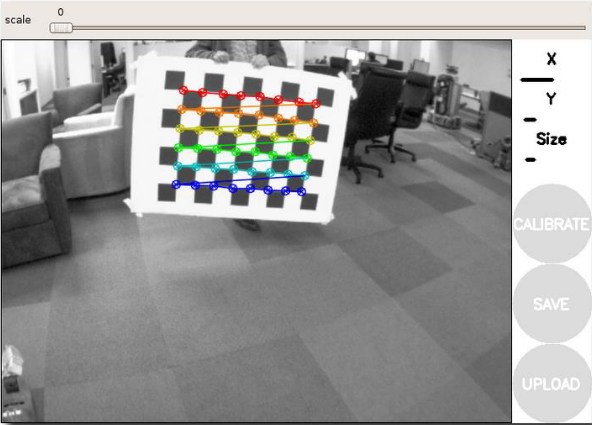
\includegraphics[width=\textwidth]{Calibration.png}    
          \caption{Exemple de calibration.}
          \label{fig:Calibration}
        \end{figure}

      \subsubsection{Recherche de chemin}
        Après avoir passé un certain temps sur le code source d'ORB-SLAM3 pour comprendre comment chaque partie fonctionnait, nous avons
        été en capacité de réfléchir à comment nous implanter dedans pour ajouter notre contribution. L'idée était d'être capable de garder
        en mémoire les lieux importants pour l'utilisateur (POI) et de lui permettre d'y retourner en trouvant le chemin le plus court
        entre la position courante et la destination voulue grâce à l'algorithme A*.    

        \paragraph{Matrice de coordonnées}
          Les coordonnées résultantes d'ORB-SLAM3 sont des nombres flottants généralement compris dans l'intervalle $[0,1]$ pour les vidéos
          courtes. Nous avions besoin d'un moyen de projeter ces coordonnées sur une grille afin de déterminer le chemin à parcourir
          et de donner des indications de direction alors il a fallu adapter le résultat fournis par ORB-SLAM3.

         La projection est assez simple, nous multiplions la coordonnée flottante de la caméra par 10, on arrondi au supérieur afin d'obtenir
         un nombre entier puis un divise le résultat par 10. Cela nous a permis d'obtenir une grille de coordonnées discrétisées qui ne soit
         pas trop petite (une grille trop petite correspondrait à des espacements plus petit qu'un pas dans le monde réel), ce qui nous permet
         de ne pas guider l'utilisateur trop souvent. Un exemple de cette méthode de discrétisation est présenté dans la Figure 
         \ref{fig:Coordonnees}.

         \begin{figure}[hbt]  
          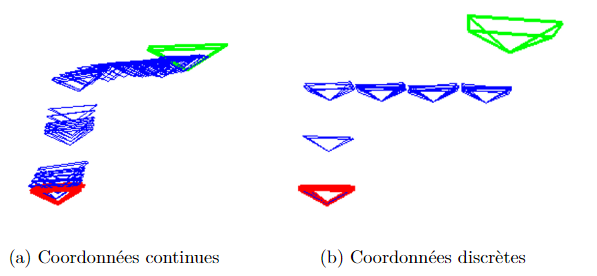
\includegraphics[width=\textwidth]{Coordonnees.png}    
          \caption{Exemple de discrétisation.}
          \label{fig:Coordonnees}
        \end{figure}  

        \paragraph{Structures de données définies}

          \subparagraph{Coord}
            Nous avons créé une structure $Coord$ en C++, équivalente à un vecteur 2D. Cette structure est utilisée par tous nos algorithmes.
            
          \subparagraph{AbsoluteCoord}
            Les coordonnées absolues sont les coordonnées the la caméra qui ont été projetées sur une grille discrète. Nous avons créé une 
            structure $AbsoluteCoord$ contenant 5 champs:

            \begin{itemize}
              \item $int$ $x_{min}$, $x_{max}$, $y_{min}$, $y_{max}$: les dimensions de la grille.
              \item $vector$<$Coord$> $coords$: Le chemin parcouru par la caméra.          
            \end{itemize}    

          \subparagraph{Path}        
            Nous avons créé une structure $Path$ contenant 2 champs: 
            \begin{itemize}
              \item $Coord$ $start$: la position courante sur la carte quand le chemin est sauvegardé, celle qui sera fournie à l'algorithme
              A* pour la recherche de chemin.
              \item $vector$<$vector<int>>$ $Map2D$: La matrice représentant les chemins explorés par l'utilisateur. Cette carte 2D est crée 
              depuis les coordonnées absolues.     
            \end{itemize} 

          \subparagraph{PoiList}   
            Nous enregistrons la liste des POI sauvegardés sous la forme d'un dictionnaire $map$<$string$, $Coord$> $poiList$ qui associe
            un nom à une position. Ce dictionnaire est mis à jour lorsque l'utilisateur demande la sauvegarde d'un endroit.            

        \paragraph{L'algorithme A*}
          L'algorithme A* est un algorithme de recherche dont le but est de trouver le plus court chemin entre 2 positions dans une matrice.
          Imaginons une grille carré contenant des obstacles répartis aléatoirement, on fourni la position de départ $A$ et la destination $B$.
          Le but est de rejoindre la destination le plus rapidement possible.
          L'algorithme A* prend 3 paramètres:

          \begin{itemize}
            \item G: Le coût de déplacement de la cellule initiale jusqu'à la cellule courante. Cela correspond à la somme de toutes les 
            cellules qui ont été visitées depuis le départ de la première cellule.
            \item H: La valeur heuristique, c'est une estimation du coût de déplacement depuis la cellule courante jusqu'à la destination. 
            Il faut faire attention à ne pas surrestimer cette valeur.
            \item F = G + H            
          \end{itemize} 
          A* base se décision sur la valeur de F, il cherche toujours à minimiser cette valeur jusqu'à atteindre sa destination,
          comme le montre la Figure \ref{fig:Astar}.          
          
          \begin{figure}[hbt]  
            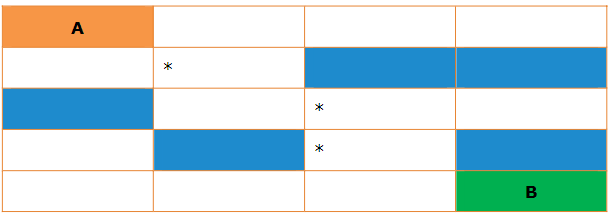
\includegraphics[width=\textwidth]{Astar.png}    
            \caption{Exemple de A*.}
            \label{fig:Astar}
          \end{figure} 


        \paragraph{Retourner à un point d'intérêt}
          Dans cette partie nous avons ajouté un bouton à l'interface graphique fournie avec ORB-SLAM3 qui affiche la liste des POI et 
          demande à l'utilisateur de choisir sa destination. La coordonnée associée à la destination choisie est donnée à A* pour trouver
          le plus court chemin pratiquable. Le chemin trouvé est ensuite donné à la fonction $FYWBack()$.          

        \paragraph{FYWBack}
            Après avoir récupéré la sortie de l'algorithme A* sous la forme d'une liste de coordonnées, $FYWBack()$ fourni des indications
            de directions en se basant sur la normale au plan de la caméra et calcule l'angle avec la section de chemin la plus proche
            afin guider l'utilisateur. Le chemin à parcourir est regénéré section par section.            
      
      \subsubsection{Test et résultats}
        Nous avons testé notre travail sur plusieurs vidéos prises dans l'openSpace. Nous avons d'abord essayé de créer une grille 2D de la 
        carte locale comme présenté dans la Figure \ref{fig:Test1}. Ensuite, nous avons calculé les normales des images clés en temps réel 
        comme présenté dans la Figure \ref{fig:Test2}. Nous avons ensuite réussi à sauvegarder une position, appellée POI, et la nommer comme
        présenté en Figure \ref{fig:Test3}. Enfin nous avons créé une fonction de retour à un POI depuis la position courante, montré dans la 
        Figure \ref{fig:Test4}.

        \begin{figure}[hbt]  
          \centering
          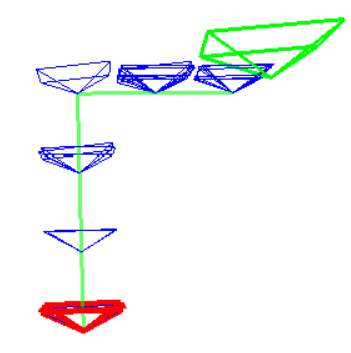
\includegraphics[width=50mm]{Test1.png}    
          \caption{Grille 2D de la carte locale.}
          \label{fig:Test1}
        \end{figure} 

        \begin{figure}[hbt]  
          \centering
          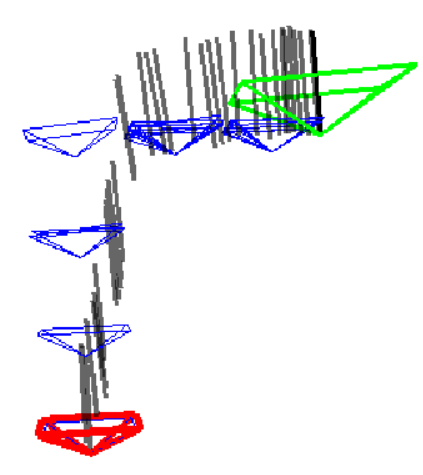
\includegraphics[width=50mm]{Test2.png}    
          \caption{Normales des images clés en temps réel.}
          \label{fig:Test2}
        \end{figure} 

        \begin{figure}[hbt]  
          \centering
          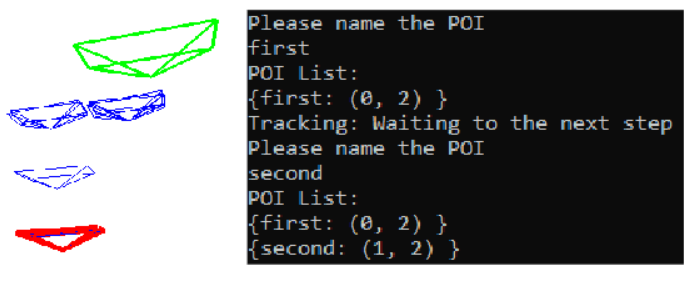
\includegraphics[width=90mm]{Test3.png}    
          \caption{Sauvegarde d'un point d'intéret.}
          \label{fig:Test3}
        \end{figure} 

        \begin{figure}[hbt]  
          \centering
          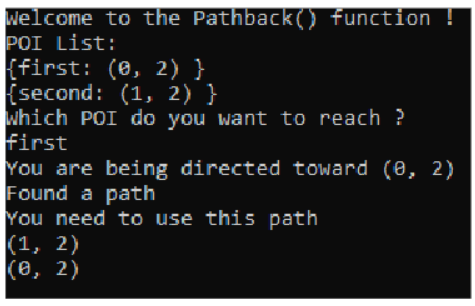
\includegraphics[width=80mm]{Test4.png}    
          \caption{Retour à un point d'intéret.}
          \label{fig:Test4}
        \end{figure}    
        
        
      \pagebreak
      \subsubsection{Difficultés rencontrées}
        Nous avons passé la majeur partie du temps qui nous était imparti pour le POC à essayer d'installer ORB-SLAM3. La recherche des bonnes
        versions pour chaque bibliothèque nous a beaucoup retardé. Certaines parties du code source ont dû être éditées, notament au niveau
        de CMakeLists.txt pour faire fonctionner le tout.
        De nombreux problèmes sont survenus concernant quasiment chaque package qu'il fallait installer, la plupart du temps à cause de
        problèmes de compatibilité ou de documentation manquante. La seule solution que nous ayons trouvé à été de chercher sans relâche jusqu'à
        trouver une solution.
        Lorsque nous travaillions sur la VM, des latences et des crash innatendus nous ont également fortement ralentis.       
 
      \subsubsection{Conclusion}
        Pour conclure sur la phase de POC, nous avons réussi à faire fonctionner un système SLAM pour la première fois chez Aubay, d'autres
        équipe ayant essayé sans succès par le passé. En plus de réussir l'installation, nous avons ajouté les fonctionnalités nécéssaires
        pour atteindre notre but et avoir un module prêt à intégrer la phase projet pour venir se lier aux autres POC de notre projet.
% TODO: Relire la phase projet.
    \subsection{Phase projet}
      Une fois la phase de \acrshort{poc} terminée, nous devions ensuite passer à la phase projet, nécéssitant d'associer nos \acrshort{poc}
      afin de créer une application de démonstration pour la \acrshort{jds} du 7 juillet 2022. Cette journée est un jalon très important
      pour tout stagiaire au sein de la cellule Innov' de chez Aubay. Elle sert à présenter le projet sur lequel chaque équipe a travaillé
      afin de montrer à la direction générale ainsi qu'aux directeur commerciaux de dont les stagiaires sont capable, et ce qu'Aubay pourrait
      proposer à ses clients dans le futur. Nous avons donc réfléchis à la création d'une application et d'une
      interface graphique nous permettant de démontrer
      le fonctionnement de notre application, bien que l'application finale soit destinée à des personnes malvoyantes, ne nécessitant pas 
      d'autre interface qu'une interface vocale.

      \subsubsection{Protocole de communication}
        Il est important de noter que nos 3 POCs ne fonctionnent pas sur les mêmes systèmes, en effet, le POC SLAM développé en C++
        fonctionne uniquement sur WSL2, tandis que les POC Computer Vision (\acrshort{cv}) et Natural Language Processing (\acrshort{nlp}) sont développés en Python 
        sur Windows. Le problème étant que WSL2 ne nous permettait pas d'accéder au flux vidéo de la caméra nécéssaire aux POCs SLAM et CV, 
        qu'une VM nous le permettait mais ne donnait pas accès aux GPU nécéssaires aux POCs CV et NLP. Nous avons optés pour trouver une 
        solution
        concernant le problème de flux vidéo sur WSL2. Étant donné que les 3 POCs devaient fonctionner sur le même réseau local, l'idée de 
        mettre
        en place un serveur Flask afin d'établir une communication entre Windows et WSL2 pour transmettre le flux vidéo de Windows à WSL2. 
        Cette solution a nécéssité d'adapter la manière dont ORB-SLAM3 récuperait le flux vidéo avant de l'incorporer à son 
        fonctionnement normal.

        L'application est composée d'un backend et d'un frontend. Le backend se charge des fonctionnalités, le frontend s'occupe du rendu
        graphique afin de présenter les résultats à l'utilisateur. La structure de l'application est simple: Les 3 POCs communiquent à un 
        chef d'orchestre pour envoyer leur requête ou récupérer le résultat d'une requête précédemment effectuée et le frontend récupère
        les résultats à afficher après avoir sélectionner le mode de démonstration adapté. Ce fonctionnement est illustré dans la 
        Figure \ref{fig:Structure}.

        \begin{figure}[hbt]  
          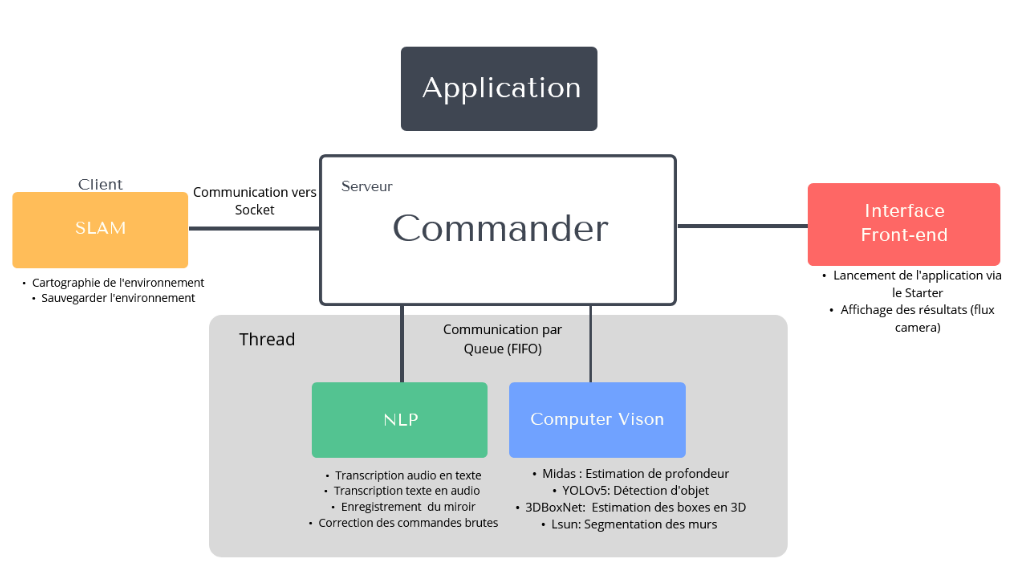
\includegraphics[width=\textwidth]{StructureApp.png}    
          \caption{Schéma présentant l'architecture de l'application.}
          \label{fig:Structure}
        \end{figure} 

        Le POC SLAM se situant sur un système différent et utilisant un langage de programmation différent des POCs CV et NLP, il a fallu
        recourir aux sockets qui sont disponible dans beaucoup de langages de programmation dont C++ et Python. Après avoir autorisé les 
        communications au niveau du proxy et du par-feu en ouvrant les bons ports, cette communication par socket a pu être réalisée.
        Une fois la communication rendue possible, il a fallu ajouter des threads au code d'ORB-SLAM3 permettant des interruptions
        pour envoyer les données nécéssaires après leur traîtement ou recevoir les instructions du chef d'orchestre
        afin d'executer les fonctions utiles au bon moment.

        % TODO: Mettre le schéma de Victor concernant la communication.

      \subsubsection{Développement de l'application}         
        L'application fonctionne avec une caméra branchée pour transmettre le flux vidéo aux différents modules s'en servant ainsi qu'avec
        un micro et un haut-parleur.  
        L'interface graphique donne la possibilité de lancer une démonstration et de démarrer les parties SLAM, CV et NLP via le serveur Flask 
        et des sockets. Cette interface a été développée avec Python grace à la bibliothèque PyQt5. La page principale de l'application est
        montrée en Figure \ref{fig:Application}, on y voit les résultats des POCs CV et SLAM ainsi que les différents boutons permettant
        à l'utilisateur d'intéragir pour tester l'application. Ces boutons servent à: 

        \begin{itemize}
          \item Lancer une vidéo de démonstration.
          \item Lancer l'application en temps réel.
          \item Utiliser le microphone pour exprimer une commande vocale lorsque l'application s'exécute en temps réel.
          \item Sauvegarder la postion courante comme un lieu favoris afin de pouvoir s'y faire guider plus tard.
          \item Demander à se faire guider à un lieu précédemment sauvegardé.
          \item Afficher l'historique des commandes utilisées et réponses reçues.   
        \end{itemize} 

        \begin{figure}[hbt]  
          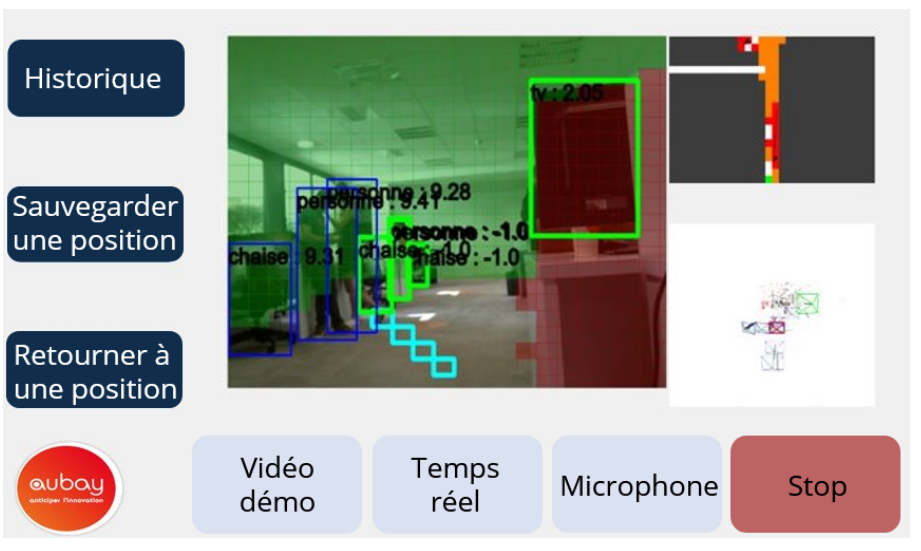
\includegraphics[width=\textwidth]{Application.png}    
          \caption{Page principale de l'application.}
          \label{fig:Application}
        \end{figure}     

  \pagebreak
  
  \section{Les dimensions humaines et managériales (3 à 5 p)}
  Les dimensions humaines et managériales internes à l’organisme d’accueil. Cette partie consiste en
  une présentation analytique des processus d’entreprise. Selon les cas, elle portera sur la conduite de
  projet, les aspects organisationnels, la gestion du changement, le travail en groupe, l’énoncé des
  objectifs individuels et de l’équipe, la contribution à l’atteinte des objectifs, les difficultés rencontrées,
  les aides reçues, etc. Les difficultés propres à l’entreprise ou au service dans lequel la mission a été
  effectuée doivent être abordées de façon professionnelle pour que le jury ait une appréciation réaliste
  des conditions du travail réalisé. 
  
  % TODO: Dimension humaine et managéiales.

  Méthode agile 
  Daily
  Comité le mardi à 14h45
  Jira pour suivre le projet et ses avancées, sprint de 2 semaines
  Scrum Master élu chaque semaine
  3 groupes de 3, 3 et 4 indépendants puis mise en commun lors de la phase projet

  \pagebreak
  
  \section{Conclusion (2 à 3 p)}
  La conclusion générale, de quelques pages, porte sur l’ensemble de votre expérience technique et
  humaine. Une première partie correspond au bilan et une deuxième partie expose les possibilités
  d’évolution du projet, du produit. Enfin, vous présenterez vos perspectives d’évolution par rapport à
  votre projet professionnel initial. Vous préciserez les compétences que vous avez développées en
  école d’ingénieurs et durant votre mission de fin d’études et préciserez vos axes d’amélioration.

  % TODO: Conclusion.

  Bilan technique sur le projet

  Possibles évolutions

  \pagebreak
  
  \section{Bibliographie}

    \printbibliography[heading=none]

  \pagebreak
  
  \section{Annexes}

    \subsection{Point d'intéret}
      Le but d'un point d'intérêt est de permettre à un algorithme de déterminer que deux objets sont bien les mêmes sur deux images 
      différentes en ayant appliqué des modifications telles qu'un changement d'échelle, une rotation, une translation ou même une 
      variation de l'intensité lumineuse.
      L'idée est donc de trouver des points caractéristiques sur les images récupérées de manière à ce que ces points décrivent au mieux 
      l'objet en cours de traîtement. En regroupant ces points caractéristiques, appellés "points d'intérêt", on est capable de déterminer 
      si deux objets avec un point de vue différent sont les même ou non. Les méthodes d'extractions de \acrshort{poi} les plus populaires 
      sont les méthodes SIFT et ORB par exemple.
      Une fois un point d'intérêt détecté, on veut être capable de résumer son information d'une manière simple afin de pouvoir le comparer
      à d'autres points d'intérêts. On peut utiliser l'intensité lumineuse ou le gradient des pixels environnants le point d'intéret pour 
      former un descripteur correcte, tout en respectant les règles de discrimination et d'invariance. Les descripteurs sont en général 
      stockés dans des vecteurs de 128 bits, ce qui permet une comparaison rapide.

      La comparaison entre deux descripteurs se fait généralement par des calculs booléens tels que présenté dans la 
      Figure \ref{fig:Descripteur}.
      
      \begin{figure}[hbt]  
        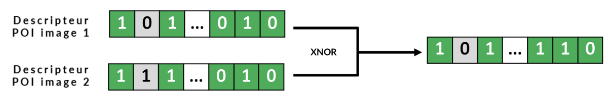
\includegraphics[width=\textwidth]{CalculsDescripteurs.png}    
        \caption{Association de descripteur avec une opération booléenne.}
        \label{fig:Descripteur}
      \end{figure} 

    \subsection{FAST}
      Cette méthode d'extraction de \acrshort{poi} vérifie pour chaque pixel de l'image d'intensité $I_p$ si au moins 12 des pixels
      du cercle autour du pixel ont une intensité supérieure ou inférieure à une proportion de $I_p$. Autrement dit on regarde si il y a une 
      grosse démarquation d'intensité entre le pixel et ses voisins comme le montre la Figure \ref{fig:CercleSuperiorite}.

      \begin{figure}[hbt]  
        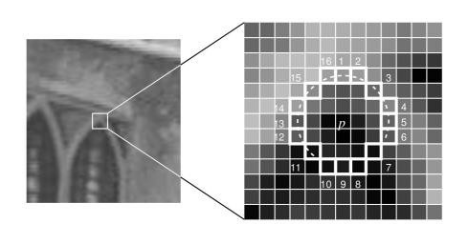
\includegraphics[width=\textwidth]{CercleSuperiorite.png}    
        \caption{Cercle de supériorité associé à un pixel.}
        \label{fig:CercleSuperiorite}
      \end{figure}

    \subsection{BRIEF}
      Des paires de pixels autour du POI sont générées aléatoirement et des tests de supériorités sont effectués dessus. 
      Un vecteur descripteur issu de la concaténation des résultats de ces tests de supériorité est créé. Un exemple est présenté 
      dans la Figure \ref{fig:Paires}.

      \begin{figure}[hbt]  
        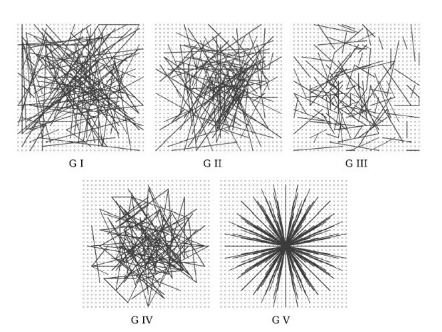
\includegraphics[width=\textwidth]{Paires.png}    
        \caption{Exemple de paires de pixels à tester.}
        \label{fig:Paires}
      \end{figure}   

      Un exemple d'appariement des POI est présenté dans la Figure \ref{fig:Appariement}. 

      \begin{figure}[hbt]  
        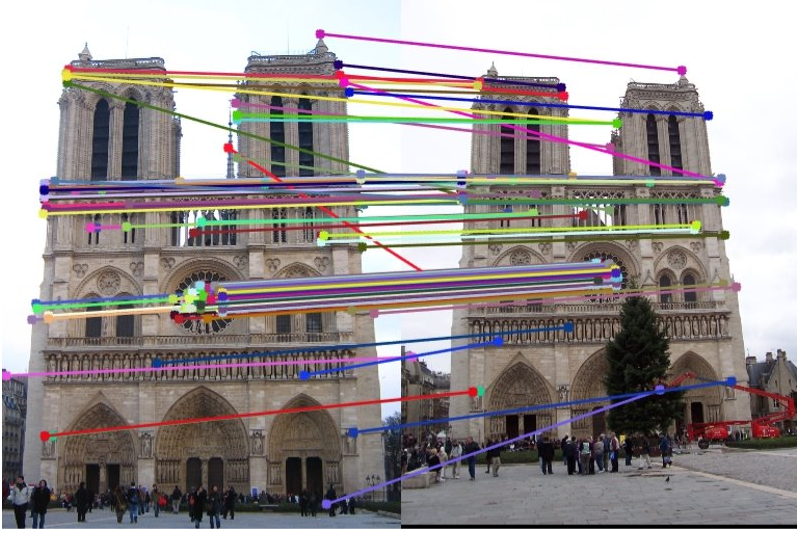
\includegraphics[width=\textwidth]{AssociationPOI.png}    
        \caption{Exemple d'association de POI.}
        \label{fig:Appariement}
      \end{figure}   
    
    \pagebreak
    \printnoidxglossary[type=acronym, nonumberlist]
    \printacronyms
 
\end{document}